% !TeX root = ../main.tex
\chapter{Unidad 10: El ruido y su caracterización}
\label{chap:unidad-10}

\section{Propósito y resultados de aprendizaje}
\label{sec:u10-proposito}

En esta unidad estudiaremos el ruido como una señal física cuya interpretación
depende también de la tarea y del contexto. El propósito no es decidir si todo
sonido es agradable o molesto, sino aprender a describir señales variables,
comparar sus contenidos temporal y frecuencial, interpretar métricas de
exposición y elegir medidas de control coherentes con cada problema.

Al finalizar la unidad se espera que podamos:
\begin{enumerate}
    \item diferenciar el fenómeno sonoro, la señal medida y la valoración
    contextual como ruido;
    \item distinguir señales determinísticas y aleatorias, y reconocer ruido
    estacionario y no estacionario;
    \item clasificar un ruido como continuo, fluctuante, intermitente o
    impulsivo a partir de su evolución temporal;
    \item calcular e interpretar valor medio, valor eficaz, varianza y nivel
    equivalente;
    \item relacionar densidad espectral, energía por banda y ruidos blanco,
    rosa, con forma espectral vocal y de banda estrecha;
    \item diferenciar nivel instantáneo, máximo, de pico y equivalente;
    \item explicar el papel de un ruido enmascarante sin confundirlo con el
    ruido de fondo ni con un protector auditivo;
    \item organizar el control del ruido en la fuente, el trayecto y el
    receptor, sin confundir reducción, absorción, aislamiento y cancelación
    activa; y
    \item reconocer qué afirmaciones sobre exposición, salud y procedimientos
    requieren una norma, una jurisdicción o un protocolo clínico específico.
\end{enumerate}

\section{Conocimientos previos}
\label{sec:u10-previos}

Esta unidad retoma:
\begin{itemize}
    \item los valores instantáneo, medio y eficaz de una señal, y los niveles
    acústicos, estudiados en la \nameref{chap:unidad-4};
    \item el análisis temporal y frecuencial, las bandas, los filtros, las
    ponderaciones y el nivel equivalente, desarrollados en la
    \nameref{chap:unidad-5};
    \item el mecanismo perceptual del enmascaramiento y la relación
    señal--ruido, explicados en la \nameref{chap:unidad-7};
    \item la diferencia entre exposición, alteración, síntoma y resultado de
    una prueba, presentada en la \nameref{chap:unidad-8}; y
    \item la propagación, el acondicionamiento, el aislamiento y las cabinas,
    tratados en la \nameref{chap:unidad-9}.
\end{itemize}

Aquí aplicaremos esos conceptos para caracterizar y controlar ruido. No
repetiremos la teoría perceptual completa ni estableceremos indicaciones
diagnósticas o terapéuticas.

\section{Situación introductoria: una misma señal, distintos problemas}
\label{sec:u10-situacion}

Imaginemos un consultorio próximo a una avenida. La presión acústica producida
por el tránsito puede registrarse con un micrófono y describirse mediante una
señal \(p(t)\), donde \(p\) es la presión acústica, expresada en pascales
(\(\mathrm{Pa}\)), y \(t\) es el tiempo, expresado en segundos
(\(\mathrm{s}\)). Esa misma señal puede:
\begin{itemize}
    \item dificultar una conversación;
    \item interferir con una medición de umbrales;
    \item resultar tolerable para una persona y molesta para otra; o
    \item no ser relevante para una tarea que utiliza señales mucho mayores.
\end{itemize}

La señal física no cambia por el nombre que le demos. Lo que cambia es la
relación entre esa señal, el receptor, la tarea y el contexto. Por eso, antes
de proponer una medición o un control, conviene preguntar: ¿qué fuente produce
la señal?, ¿cómo llega al receptor?, ¿durante cuánto tiempo?, ¿en qué
frecuencias concentra energía? y ¿qué actividad se intenta proteger?

\section{Sonido y ruido: fenómeno, señal y contexto}
\label{sec:u10-sonido-ruido}

El \textbf{sonido} es un fenómeno físico asociado con perturbaciones mecánicas
que se propagan en un medio material. Un micrófono transforma una parte de ese
fenómeno en una señal eléctrica que puede medirse y analizarse.

La palabra \textbf{ruido} admite varios usos compatibles, pero no idénticos:
\begin{description}
    \item[\textbf{Uso contextual:}] sonido no deseado, molesto o que interfiere
    con una actividad.
    \item[\textbf{Uso físico y de señales:}] componente aleatoria o no deseada
    que se superpone a una señal de interés.
    \item[\textbf{Uso operativo:}] señal empleada deliberadamente para una
    medición, una prueba o una acción de control, como un ruido de banda
    estrecha utilizado como enmascarante.
\end{description}

Así, un ruido enmascarante puede ser deseado por quien realiza una prueba,
aunque interfiera de manera controlada con otra señal. Del mismo modo, una
conversación puede funcionar como ruido respecto de una tarea de atención,
sin dejar de ser habla para sus participantes. Llamar ruido a una señal no
describe por sí solo su nivel, su espectro, su duración ni sus efectos.

\section{Señales determinísticas y aleatorias}
\label{sec:u10-deterministicas-aleatorias}

Una señal es \textbf{determinística} cuando un modelo y sus parámetros permiten
predecir su valor en cada instante. Una sinusoide ideal de amplitud, frecuencia
y fase conocidas es un ejemplo. Esto no significa que toda señal
determinística sea simple: una suma conocida de muchas componentes también
puede serlo.

Una señal es \textbf{aleatoria} cuando sus valores instantáneos no pueden
predecirse exactamente y se describe mediante propiedades estadísticas. Cada
registro temporal concreto se denomina \textbf{realización}. Dos realizaciones
de un mismo proceso aleatorio no tienen que coincidir muestra por muestra,
aunque pueden compartir valor eficaz, distribución y densidad espectral.

La separación no depende de que la señal ``parezca desordenada''. Una secuencia
pseudoaleatoria generada por un algoritmo puede repetirse exactamente si se
conservan el algoritmo, los parámetros y la semilla. Resulta útil como señal de
ensayo, aunque modele ciertas propiedades de un proceso aleatorio.

\subsection{Ruido estacionario y no estacionario}
\label{sec:u10-estacionariedad}

En un proceso \textbf{estacionario}, las propiedades estadísticas elegidas no
cambian al desplazar la ventana de observación en el tiempo. En esta unidad
usaremos una interpretación práctica: media, varianza y contenido espectral
permanecen aproximadamente estables durante el intervalo analizado.

Un proceso es \textbf{no estacionario} cuando esas propiedades cambian. El
tránsito que alterna períodos calmos con el paso de vehículos, el arranque de
un equipo y una secuencia de golpes son ejemplos posibles. La clasificación
siempre depende de la escala temporal: una señal puede parecer estable durante
\(2\,\mathrm{s}\) y no serlo durante \(20\,\mathrm{min}\).

\section{Clasificación según la evolución temporal}
\label{sec:u10-clasificacion-temporal}

Las categorías temporales describen patrones observables; no identifican por
sí solas una fuente ni predicen un efecto clínico.

\begin{description}
    \item[\textbf{Continuo:}] está presente sin pausas relevantes durante el
    intervalo de interés. Puede ser estable o variar.
    \item[\textbf{Fluctuante:}] está presente, pero su nivel cambia de manera
    apreciable con el tiempo, sin períodos de ausencia claramente separados.
    \item[\textbf{Intermitente:}] alterna períodos en los que la fuente o la
    señal son identificables con otros en los que cesan o disminuyen de manera
    marcada.
    \item[\textbf{Impulsivo:}] contiene eventos breves con cambios rápidos y
    niveles de pico destacados respecto del entorno.
\end{description}

Un ruido puede pertenecer a más de una descripción. Por ejemplo, una máquina
puede producir un ruido continuo y fluctuante, mientras que una serie de
impactos puede ser impulsiva e intermitente. Los límites cuantitativos que una
norma utilice para estas categorías dependen del documento, su edición y su
finalidad; no existe una duración universal que resuelva todos los casos.

La figura~\ref{fig:u10-realizaciones-temporales} permite comparar las cuatro
categorías con los mismos ejes. Debe observarse el patrón temporal completo,
no una muestra aislada.

% Texto alternativo: cuatro registros sintéticos de presión entre 0 s y 1 s.
% El continuo estable conserva una dispersión semejante; el fluctuante cambia
% gradualmente de amplitud; el intermitente alterna actividad y pausas; el
% impulsivo presenta tres picos breves sobre un fondo pequeño.
\begin{figure}[htbp]
    \centering
    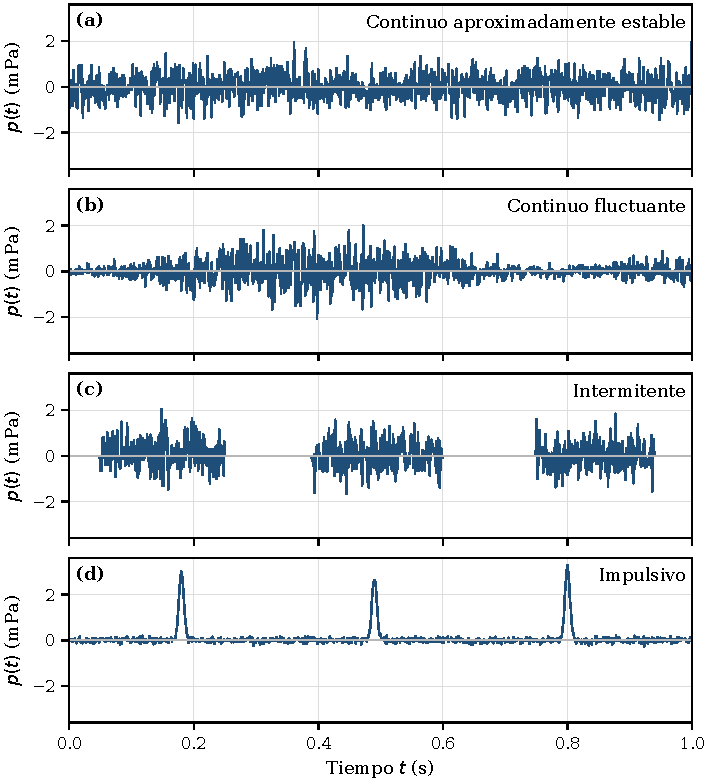
\includegraphics[width=0.96\textwidth]
        {figures/generated/unidad-10/realizaciones-temporales-ruido.pdf}
    \caption{Clasificación temporal mediante cuatro realizaciones sintéticas
    de presión acústica, muestreadas a \(1000\,\mathrm{Hz}\) durante
    \(1\,\mathrm{s}\). Los paneles comparten las escalas de tiempo y presión:
    (a)~continuo aproximadamente estable; (b)~continuo fluctuante;
    (c)~intermitente; y (d)~impulsivo. Las amplitudes ilustran la forma
    temporal y no representan una exposición medida. Elaboración propia con
    semilla fija.}
    \label{fig:u10-realizaciones-temporales}
\end{figure}

\section{Descripción estadística}
\label{sec:u10-estadistica}

Cuando una señal varía, una sola muestra no representa el intervalo completo.
Primero observamos qué pregunta responde cada descriptor y luego introducimos
su expresión matemática.

\subsection{Valor medio, valor eficaz y varianza}

Supongamos que se registran \(N\) muestras de presión acústica
\(p_1,p_2,\ldots,p_N\), todas expresadas en pascales (\(\mathrm{Pa}\)). El
\textbf{valor medio} se define como
\begin{equation}
    \overline{p}=\frac{1}{N}\sum_{i=1}^{N}p_i,
    \label{eq:u10-media}
\end{equation}
donde \(i\) identifica cada muestra. El valor medio conserva el signo. En una
señal acústica alternante medida respecto de la presión atmosférica, los
valores positivos y negativos suelen compensarse, de modo que
\(\overline{p}\) puede ser cercano a \(0\,\mathrm{Pa}\) aunque la señal
transporte energía.

El \textbf{valor eficaz} o RMS cuantifica el tamaño cuadrático de la señal:
\begin{equation}
    p_{\mathrm{rms}}=
    \sqrt{\frac{1}{N}\sum_{i=1}^{N}p_i^2},
    \label{eq:u10-rms}
\end{equation}
donde \(p_{\mathrm{rms}}\) se expresa en pascales (\(\mathrm{Pa}\)). Este valor
es el que se relaciona con el nivel de presión sonora bajo las condiciones
estudiadas en la \nameref{chap:unidad-4}.

La \textbf{varianza} describe la dispersión respecto del valor medio:
\begin{equation}
    \sigma_p^2=
    \frac{1}{N}\sum_{i=1}^{N}\left(p_i-\overline{p}\right)^2,
    \label{eq:u10-varianza}
\end{equation}
donde \(\sigma_p^2\) se expresa en pascales cuadrados
(\(\mathrm{Pa^2}\)). Para estas definiciones,
\begin{equation}
    p_{\mathrm{rms}}^2=\sigma_p^2+\overline{p}^{\,2}.
    \label{eq:u10-identidad-estadistica}
\end{equation}
Por lo tanto, si \(\overline{p}=0\,\mathrm{Pa}\), el cuadrado del valor eficaz
coincide con la varianza, pero los conceptos no son sinónimos.

\paragraph{Ejemplo.}
Consideremos cinco muestras sintéticas:
\(-2,-1,0,1,2\,\mathrm{mPa}\), donde
\(1\,\mathrm{mPa}=10^{-3}\,\mathrm{Pa}\). Su valor medio es
\(0\,\mathrm{mPa}\). El promedio de los cuadrados es
\(2\,\mathrm{mPa^2}\), por lo que
\(p_{\mathrm{rms}}=\sqrt{2}\,\mathrm{mPa}\approx1{,}41\,\mathrm{mPa}\) y
\(\sigma_p^2=2\,\mathrm{mPa^2}\). La media nula no implica ausencia de señal.

\subsection{Distribución e histograma}

La \textbf{distribución} describe con qué frecuencia o probabilidad aparecen
los distintos valores. En un registro finito puede aproximarse mediante un
histograma: se divide el eje de amplitud en intervalos y se cuenta cuántas
muestras caen en cada uno. La distribución aporta información que el RMS no
conserva. Dos señales pueden tener igual valor eficaz y, sin embargo, diferir
en la frecuencia con la que presentan valores extremos.

No debe suponerse que todo ruido posee una distribución normal o gaussiana.
Esa distribución es un modelo posible que debe comprobarse o declararse, no
una consecuencia de llamar ruido a la señal.

La figura~\ref{fig:u10-estadistica-mismo-rms} muestra por qué media, RMS y
varianza no agotan la descripción de una señal: dos registros pueden compartir
esos valores y poseer distribuciones diferentes.

% Texto alternativo: dos señales sintéticas tienen media 0 mPa, RMS 1 mPa y
% varianza 1 mPa². La señal A recorre valores continuos concentrados alrededor
% de cero; la B alterna exclusivamente -1 mPa y +1 mPa. Los histogramas hacen
% visible la diferencia que no expresan los tres descriptores compartidos.
\begin{figure}[htbp]
    \centering
    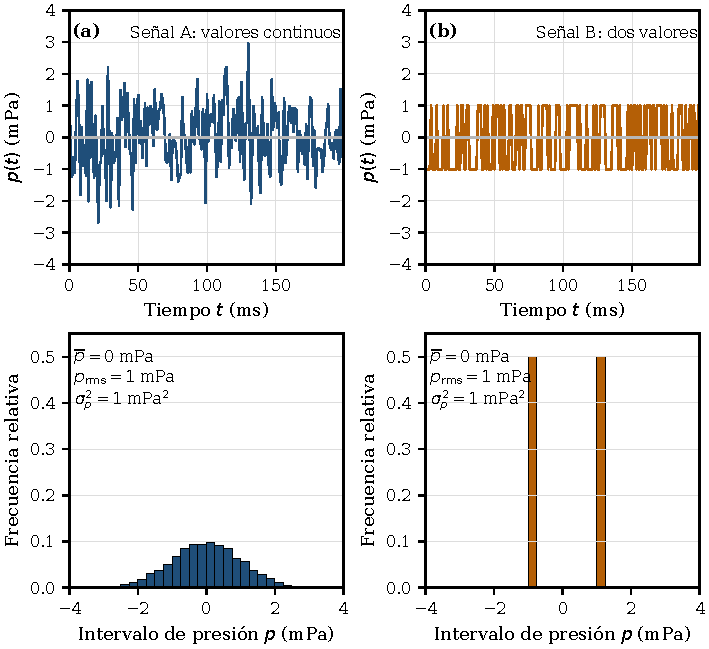
\includegraphics[width=0.96\textwidth]
        {figures/generated/unidad-10/estadistica-mismo-rms.pdf}
    \caption{Fragmentos temporales e histogramas de dos señales sintéticas de
    \(5000\) muestras a \(1000\,\mathrm{Hz}\). Ambas poseen
    \(\overline p=0\,\mathrm{mPa}\),
    \(p_{\mathrm{rms}}=1\,\mathrm{mPa}\) y
    \(\sigma_p^2=1\,\mathrm{mPa^2}\), pero la señal A adopta valores continuos
    y la B solo \(-1\,\mathrm{mPa}\) y \(+1\,\mathrm{mPa}\). El histograma
    utiliza todas las muestras; el registro muestra los primeros
    \(200\,\mathrm{ms}\). Elaboración propia con semilla fija.}
    \label{fig:u10-estadistica-mismo-rms}
\end{figure}

\section{Descripción frecuencial}
\label{sec:u10-densidad-espectral}

El espectro estudiado en la \nameref{chap:unidad-5} permite preguntar cómo
se reparte el contenido de una señal entre frecuencias. Para un proceso
aleatorio resulta útil la \textbf{densidad espectral de potencia de la presión},
que denotaremos \(S_{pp}(f)\). Usaremos una densidad unilateral, definida para
frecuencias no negativas. Aquí \(f\) es la frecuencia, expresada en hertz
(\(\mathrm{Hz}\)), y \(S_{pp}\) se expresa en \(\mathrm{Pa^2/Hz}\).

En el modelo ideal, el valor cuadrático medio contenido entre una frecuencia
inferior \(f_L\) y una frecuencia superior \(f_H\), ambas en hertz, es
\begin{equation}
    p_{B,\mathrm{rms}}^2=
    \int_{f_L}^{f_H}S_{pp}(f)\,\mathrm{d}f,
    \label{eq:u10-psd-banda}
\end{equation}
donde \(p_{B,\mathrm{rms}}\), expresado en pascales, es el valor eficaz de la
señal limitada a esa banda. La densidad no es un nivel en decibeles y tampoco
es, por sí sola, la energía total de una banda: debe integrarse sobre un ancho
de banda.

\paragraph{Ejemplo sintético.}
Si \(S_{pp}(f)=4{,}0\times10^{-8}\,\mathrm{Pa^2/Hz}\) en una banda de
\(100\,\mathrm{Hz}\), entonces
\(p_{B,\mathrm{rms}}^2=4{,}0\times10^{-6}\,\mathrm{Pa^2}\) y
\(p_{B,\mathrm{rms}}=2{,}0\times10^{-3}\,\mathrm{Pa}\). Con la referencia
\(p_0=20\,\mathrm{\mu Pa}\) usada para el aire, ese valor corresponde a
\(L_p=40\,\mathrm{dB\,SPL}\). El ejemplo describe una señal sintética; no es
un límite de exposición.

\subsection{Ruido blanco: densidad constante por hertz}
\label{sec:u10-ruido-blanco}

En un intervalo de frecuencias especificado, un \textbf{ruido blanco} ideal
posee densidad espectral constante:
\begin{equation}
    S_{pp}(f)=S_0,
    \label{eq:u10-blanco}
\end{equation}
donde \(S_0\) es una constante expresada en
\(\mathrm{Pa^2/Hz}\). Por la ecuación~\eqref{eq:u10-psd-banda}, dos bandas con
el mismo ancho en hertz contienen el mismo valor cuadrático medio.

Una octava superior abarca más hertz que una octava inferior. Por eso un ruido
blanco no entrega igual contenido a cada octava. Además, ninguna fuente real
mantiene densidad constante desde frecuencia cero hasta frecuencia infinita:
siempre deben declararse la banda de generación, la banda de medición y las
limitaciones del sistema.

\subsection{Ruido rosa: contenido constante por octava}
\label{sec:u10-ruido-rosa}

En una banda especificada, un \textbf{ruido rosa} ideal se modela mediante
\begin{equation}
    S_{pp}(f)=\frac{K}{f},
    \label{eq:u10-rosa}
\end{equation}
donde \(K\) es una constante con las unidades necesarias para que
\(S_{pp}\) se exprese en \(\mathrm{Pa^2/Hz}\); por lo tanto, \(K\) se expresa
en pascales cuadrados (\(\mathrm{Pa^2}\)). Entre una frecuencia \(f_1\) y
su doble \(2f_1\), que delimitan una octava,
\begin{equation}
    \int_{f_1}^{2f_1}\frac{K}{f}\,\mathrm{d}f=K\ln 2.
    \label{eq:u10-rosa-octava}
\end{equation}
El resultado no depende de \(f_1\): la integral tiene el mismo valor en cada
octava ideal. Esta es la diferencia central. En el modelo blanco la densidad
es constante por hertz. En el modelo rosa, el contenido es constante por
octava. La descripción aproximada de
\(-3\,\mathrm{dB}\) por octava se refiere a la densidad espectral expresada
en escala logarítmica, no a una disminución del nivel total de cada octava.

La figura~\ref{fig:u10-blanco-rosa-bandas} conecta las densidades con la
integral de la ecuación~\eqref{eq:u10-psd-banda}. La diferencia por hertz se
traduce en una diferencia clara al sumar por octavas.

% Texto alternativo: a la izquierda, la densidad blanca es horizontal y la
% rosa decrece como 1/f entre 125 Hz y 8000 Hz. A la derecha, seis grupos de
% barras representan octavas sucesivas: el contenido blanco se duplica en
% cada banda y el rosa permanece constante; ambos se normalizan por la primera.
\begin{figure}[htbp]
    \centering
    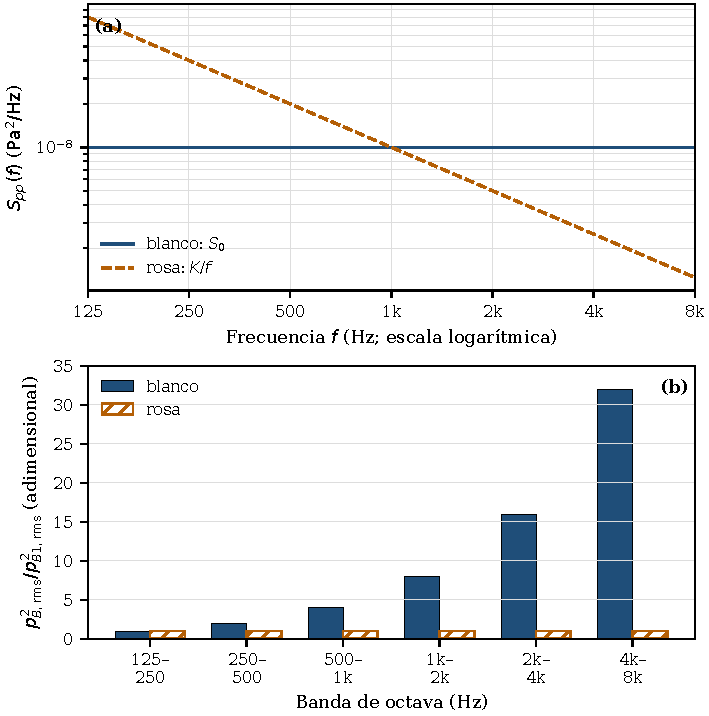
\includegraphics[width=0.98\textwidth]
        {figures/generated/unidad-10/blanco-rosa-energia-bandas.pdf}
    \caption{Modelos analíticos de ruido blanco y rosa en la banda
    \(125\)--\(8000\,\mathrm{Hz}\). (a)~Densidades
    \(S_{pp}(f)=S_0\), con
    \(S_0=1{,}0\times10^{-8}\,\mathrm{Pa^2/Hz}\), y
    \(S_{pp}(f)=K/f\), con \(K=1{,}0\times10^{-5}\,\mathrm{Pa^2}\).
    (b)~Valor cuadrático medio integrado en cada octava y normalizado por la
    primera banda: el blanco aumenta con el ancho en hertz y el rosa permanece
    constante. Son modelos finitos, no mediciones. Elaboración propia.}
    \label{fig:u10-blanco-rosa-bandas}
\end{figure}

\subsection{Ruido con forma espectral vocal}
\label{sec:u10-ruido-vocal}

El \textbf{ruido con forma espectral vocal} es una señal aleatoria filtrada
para aproximar una distribución frecuencial de referencia asociada con el
habla. No existe una única forma que pueda deducirse de su nombre: deben
especificarse el espectro objetivo, el ancho de banda, el nivel y el equipo que
lo genera.

Las denominaciones, tolerancias y usos audiométricos de los ruidos con
forma espectral vocal dependen de la norma, del transductor, del audiómetro y
del procedimiento aplicable. Una fuente normativa o documentación técnica
vigente debe acompañar cualquier especificación cuantitativa~\cite{iso389_4_1994,iec60645_1_2017}.

\subsection{Ruido de banda estrecha}
\label{sec:u10-nbn}

Un \textbf{ruido de banda estrecha} o NBN, por la sigla inglesa de
\emph{narrow-band noise}, concentra su contenido alrededor de una frecuencia
central \(f_c\), expresada en hertz. Para caracterizarlo se deben declarar la
frecuencia límite inferior \(f_L\), la frecuencia límite superior \(f_H\) y el
ancho de banda
\begin{equation}
    B=f_H-f_L,
    \label{eq:u10-ancho-nbn}
\end{equation}
donde \(B\) se expresa en hertz. También importa la pendiente del filtro fuera
de la banda. ``Banda estrecha'' no significa universalmente un tercio de
octava.

En audiometría tonal pueden emplearse ruidos de banda estrecha como
señales enmascarantes, pero sus bandas efectivas, calibración y presentación
deben corresponder al equipo, al transductor y al procedimiento vigente~\cite{iso389_4_1994,iec60645_1_2017}.

En el esquema siguiente, \(H_v(f)\) es la respuesta en frecuencia del filtro
que produce el ruido con forma espectral vocal y \(H_B(f)\) la del filtro que
produce el NBN. Se representan sus magnitudes adimensionales
\(\lvert H_v(f)\rvert\) y \(\lvert H_B(f)\rvert\) de manera cualitativa: las
curvas muestran una forma relativa, no una ganancia ni un nivel calibrados.
La figura~\ref{fig:u10-conformacion-espectral} resume qué transforma a un
ruido de banda ancha en cada una de estas señales y qué información debe
acompañar su nombre.

% Texto alternativo: dos cadenas parten de ruido de banda ancha. La superior
% atraviesa un filtro con respuesta objetivo especificada y produce ruido con
% forma espectral vocal. La inferior atraviesa un pasa banda delimitado por
% f_L y f_H, centrado en f_c, y produce ruido de banda estrecha.
\begin{figure}[htbp]
    \centering
    % Propósito: distinguir una conformación espectral de referencia de una banda
% estrecha y mostrar qué parámetros deben especificarse en cada caso.
% Origen: definiciones de las secciones \ref{sec:u10-ruido-vocal} y
% \ref{sec:u10-nbn}; B=f_H-f_L, ecuación \eqref{eq:u10-ancho-nbn}.
% Curvas y bloques cualitativos; no representan una norma ni un equipo.
% Descripción accesible: dos cadenas parten de ruido de banda ancha. La cadena
% superior atraviesa un filtro cuya respuesta H_v(f) posee una magnitud
% objetivo especificada y produce ruido con forma espectral vocal. La inferior
% atraviesa un filtro pasa banda de respuesta H_B(f), delimitado por f_L y
% f_H, centrado en f_c, y produce NBN.
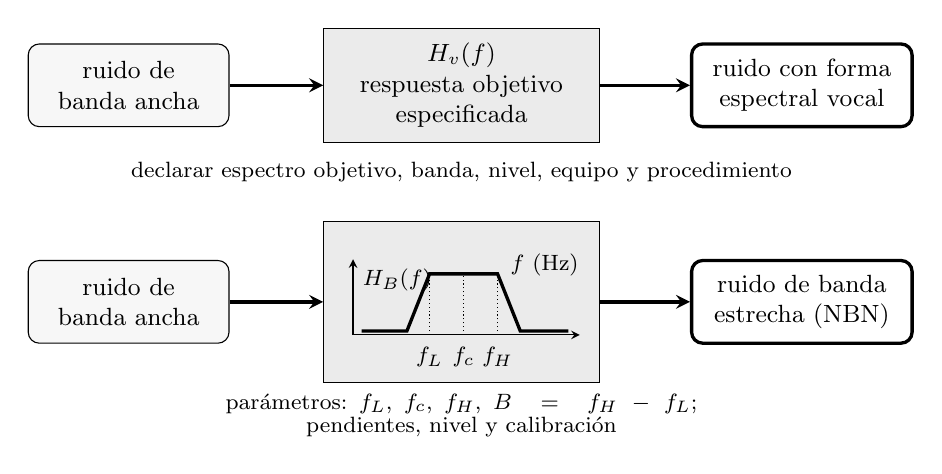
\begin{tikzpicture}[
    x=0.95cm,
    y=1cm,
    >=stealth,
    font=\small,
    bloque/.style={
        draw,
        rounded corners,
        minimum width=2.55cm,
        minimum height=1.05cm,
        align=center,
        fill=black!3
    },
    filtro/.style={
        draw,
        minimum width=3.50cm,
        minimum height=1.45cm,
        align=center,
        fill=black!8
    },
    salida/.style={
        draw,
        rounded corners,
        minimum width=2.80cm,
        minimum height=1.05cm,
        align=center,
        very thick
    }
]
    \node[bloque] (entrada-v) at (1.55,4.65)
        {ruido de\\banda ancha};
    \node[filtro] (filtro-v) at (6.00,4.65)
        {\(\lvert H_v(f)\rvert\)\\
         respuesta objetivo\\especificada};
    \node[salida] (salida-v) at (10.55,4.65)
        {ruido con forma\\espectral vocal};
    \draw[->,very thick] (entrada-v) -- (filtro-v);
    \draw[->,very thick] (filtro-v) -- (salida-v);

    \node[align=center,font=\footnotesize,text width=8.4cm]
        at (6.00,3.55)
        {declarar espectro objetivo, banda, nivel, equipo y procedimiento};

    \node[bloque] (entrada-b) at (1.55,1.90)
        {ruido de\\banda ancha};
    \node[filtro,minimum height=2.05cm] (filtro-b) at (6.00,1.90) {};
    \node[salida] (salida-b) at (10.55,1.90)
        {ruido de banda\\estrecha (NBN)};
    \draw[->,very thick] (entrada-b) -- (filtro-b);
    \draw[->,very thick] (filtro-b) -- (salida-b);

    \begin{scope}[shift={(4.55,1.48)},x=0.72cm,y=0.62cm]
        \draw[->] (0,0) -- (4.00,0);
        \node[font=\footnotesize] at (3.38,1.43)
            {\(f\) (Hz)};
        \draw[->] (0,0) -- (0,1.55);
        \node[below right,font=\footnotesize] at (0,1.55)
            {\(\lvert H_B(f)\rvert\)};
        \draw[very thick]
            (0.15,0.08) -- (0.95,0.08) -- (1.35,1.25) --
            (2.55,1.25) -- (2.95,0.08) -- (3.80,0.08);
        \draw[densely dotted] (1.35,0) -- (1.35,1.25);
        \draw[densely dotted] (1.95,0) -- (1.95,1.25);
        \draw[densely dotted] (2.55,0) -- (2.55,1.25);
        \node[below=1pt,font=\footnotesize] at (1.35,0) {\(f_L\)};
        \node[below=1pt,font=\footnotesize] at (1.95,0) {\(f_c\)};
        \node[below=1pt,font=\footnotesize] at (2.55,0) {\(f_H\)};
    \end{scope}

    \node[align=center,font=\footnotesize,text width=10.0cm]
        at (6.00,0.46)
        {parámetros: \(f_L,\ f_c,\ f_H,\ B=f_H-f_L\);\\[-1pt]
         pendientes, nivel y calibración};
\end{tikzpicture}

    \caption{Conformación espectral de dos señales de ruido.
    En la cadena superior, \(\lvert H_v(f)\rvert\) representa la magnitud de la
    respuesta objetivo que produce el ruido con forma espectral vocal; el
    nombre no define una curva universal. En la inferior,
    \(\lvert H_B(f)\rvert\) representa la magnitud de la respuesta pasa banda
    que produce el NBN, para el cual deben declararse \(f_L\), \(f_c\), \(f_H\),
    el ancho \(B=f_H-f_L\), las pendientes, el nivel y la calibración. Esquema
    cualitativo de elaboración propia; no reproduce una norma ni un equipo.}
    \label{fig:u10-conformacion-espectral}
\end{figure}

\section{Descriptores temporales y métricas de exposición}
\label{sec:u10-metricas}

Una lectura de nivel solo es interpretable si se informa qué operación se
realizó, con qué ponderación frecuencial y durante qué intervalo. La
instrumentación básica y las ponderaciones A, C y Z se estudiaron en la
\nameref{chap:unidad-5}. Aquí comparamos las preguntas que responden los
descriptores más frecuentes.

En la tabla, todos los niveles se expresan en decibeles (\(\mathrm{dB}\)) con
el calificador que corresponda, por ejemplo \(\mathrm{dB(A)}\) o
\(\mathrm{dB\,SPL}\).

\begin{center}
\small
\begin{tabular}{|
    >{\raggedright\arraybackslash}p{0.22\textwidth}|
    >{\raggedright\arraybackslash}p{0.32\textwidth}|
    >{\raggedright\arraybackslash}p{0.34\textwidth}|}
    \hline
    \textbf{Descriptor} & \textbf{Qué representa} &
    \textbf{Qué debe acompañarlo} \\
    \hline
    \(L(t)\) & Nivel indicado en un instante por el detector elegido. &
    Ponderación frecuencial y respuesta temporal. \\
    \hline
    \(L_{\mathrm{max}}\) & Mayor nivel indicado durante el intervalo. &
    Ponderaciones frecuencial y temporal e intervalo de búsqueda. \\
    \hline
    \(L_{\mathrm{peak}}\) & Nivel asociado con el mayor valor absoluto
    instantáneo de presión captado por un detector de pico. &
    Ponderación frecuencial, rango del equipo y procedimiento. \\
    \hline
    \(L_{\mathrm{eq},T}\) & Nivel constante que posee el mismo promedio
    cuadrático que la señal variable durante \(T\). &
    Duración \(T\), ponderación frecuencial y condiciones de medición. \\
    \hline
    \(L_{n,T}\) & Nivel excedido durante el \(n\)~\% del intervalo \(T\). &
    Valor de \(n\), duración, ponderación y criterio de muestreo. \\
    \hline
    Exposición o dosis & Agregación de nivel y duración para compararla con
    un criterio. & Norma, edición, jurisdicción, población y regla de
    intercambio. \\
    \hline
\end{tabular}
\end{center}

El nivel máximo no es necesariamente el nivel de pico. El primero depende de
la respuesta temporal del instrumento; el segundo intenta representar un
extremo de la presión instantánea. La ponderación temporal \emph{Impulse}
tampoco convierte automáticamente una lectura en \(L_{\mathrm{peak}}\).

El nivel equivalente no es un promedio aritmético de niveles en decibeles. Si
se dispone de \(M\) intervalos de igual duración con niveles equivalentes
\(L_1,L_2,\ldots,L_M\), todos expresados con la misma referencia y
ponderación, se obtiene
\begin{equation}
    L_{\mathrm{eq}}=
    10\log_{10}\left(
    \frac{1}{M}\sum_{j=1}^{M}10^{L_j/10}
    \right),
    \label{eq:u10-leq-intervalos}
\end{equation}
donde \(j\) identifica cada intervalo.

\paragraph{Ejemplo.}
Cuatro intervalos consecutivos de \(15\,\mathrm{min}\) poseen niveles
equivalentes ponderados A de \(88\), \(92\), \(86\) y \(90\,\mathrm{dB(A)}\).
Como las duraciones son iguales,
\[
L_{A\mathrm{eq},1\,\mathrm{h}}=
10\log_{10}\left(
\frac{10^{88/10}+10^{92/10}+10^{86/10}+10^{90/10}}{4}
\right)
\approx89{,}6\,\mathrm{dB(A)}.
\]
El resultado resume el promedio cuadrático ponderado A durante una hora; no
informa por sí solo el máximo ni el pico.

Los percentiles tampoco poseen una interpretación universal. En
\(L_{n,T}\), el subíndice \(n\) representa el porcentaje de excedencia y no es
una abreviatura de ruido. \(L_{10,T}\) es el nivel excedido durante el
\(10\)~\% de \(T\), y
\(L_{90,T}\), el excedido durante el \(90\)~\%. En algunos contextos el
segundo se usa como descriptor del ambiente residual, pero no debe llamarse
automáticamente ``ruido de fondo'' sin definir el procedimiento.

La normalización de una exposición a una jornada de referencia, el
cálculo de dosis y la combinación de protección auditiva dependen del criterio
normativo vigente. No deben mezclarse valores procedentes de organismos,
ediciones o jurisdicciones diferentes~\cite{nioshNoise1998,argentinaDecreto351}.

\section{Relación señal--ruido y ruido de fondo}
\label{sec:u10-snr-fondo}

La \textbf{señal de interés} es la componente que se intenta detectar, medir o
comprender. El \textbf{ruido de fondo} reúne las componentes no deseadas
presentes en el entorno o en la cadena de medición. En cambio, una
\textbf{señal enmascarante} se introduce deliberadamente para modificar la
detectabilidad de otra señal. Un mismo tipo espectral puede cumplir funciones
diferentes según cómo se lo utilice.

Para niveles compatibles y medidos en condiciones comparables, una forma
simple de expresar la relación señal--ruido es
\begin{equation}
    \mathrm{SNR}=L_{\text{señal}}-L_{\text{ruido}},
    \label{eq:u10-snr}
\end{equation}
donde \(L_{\text{señal}}\) es el nivel de la señal,
\(L_{\text{ruido}}\) el nivel del ruido y la SNR se expresa en decibeles
(\(\mathrm{dB}\)). Por ejemplo, si
\(L_{\text{señal}}=65\,\mathrm{dB\,SPL}\) y
\(L_{\text{ruido}}=58\,\mathrm{dB\,SPL}\), ambos medidos en la misma banda y
posición, entonces \(\mathrm{SNR}=7\,\mathrm{dB}\).

La SNR física no es una medida directa de inteligibilidad, molestia ni
esfuerzo auditivo. Esos resultados dependen además del espectro, el tiempo, el
entorno, la tarea y el oyente, como se analizó en la
\nameref{chap:unidad-7}.

La figura~\ref{fig:u10-snr-sintetica} mantiene fija la señal de interés y
modifica solo el RMS del ruido. Así se observa qué significa reducir la SNR
sin convertirla en una predicción perceptual.

% Texto alternativo: tres mezclas contienen la misma señal sintética y la misma
% realización de ruido, escalada para SNR de +12 dB, 0 dB y -6 dB. La mezcla
% sigue de cerca la señal limpia en el primer panel y se aparta cada vez más
% en los dos siguientes.
\begin{figure}[htbp]
    \centering
    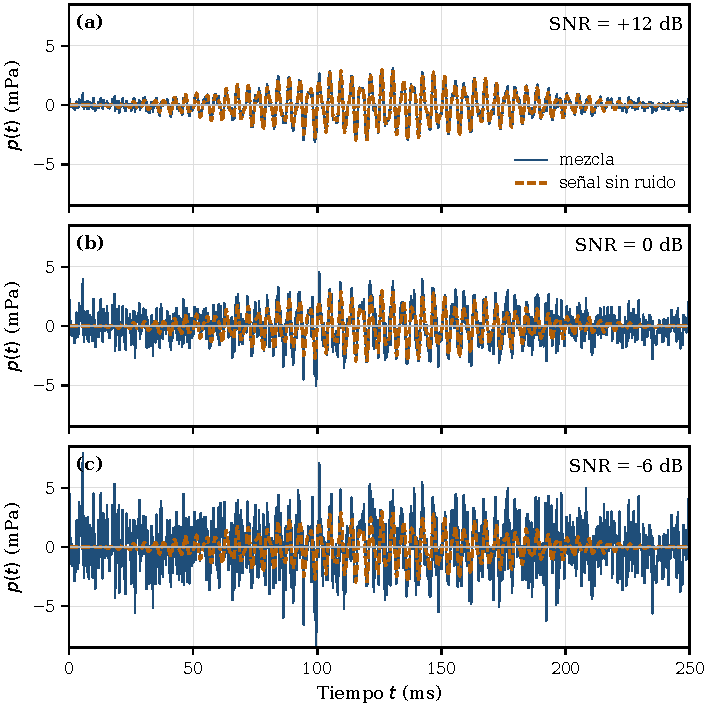
\includegraphics[width=0.96\textwidth]
        {figures/generated/unidad-10/relaciones-senal-ruido.pdf}
    \caption{Una señal sintética de \(250\,\mathrm{ms}\), formada por
    componentes de \(240\,\mathrm{Hz}\) y \(430\,\mathrm{Hz}\) bajo una
    envolvente suave, se suma a la misma realización de ruido con tres escalas:
    (a)~\(\mathrm{SNR}=+12\,\mathrm{dB}\);
    (b)~\(\mathrm{SNR}=0\,\mathrm{dB}\); y
    (c)~\(\mathrm{SNR}=-6\,\mathrm{dB}\). La señal posee
    \(p_{\mathrm{rms}}=1\,\mathrm{mPa}\); el ruido se ajusta por RMS para
    alcanzar cada relación. No son registros de habla ni mediciones.
    Elaboración propia con semilla fija.}
    \label{fig:u10-snr-sintetica}
\end{figure}

\section{Enmascaramiento: del fenómeno perceptual a la aplicación}
\label{sec:u10-enmascaramiento-aplicado}

El enmascaramiento es la disminución de detectabilidad de una señal debido a
otra. La elevación de umbral, las bandas auditivas y las dependencias
frecuencial y temporal pertenecen a la \nameref{chap:unidad-7}. En esta
unidad nos concentramos en describir la señal utilizada como enmascarante.

En una situación controlada conviene identificar:
\begin{enumerate}
    \item la \textbf{señal de prueba};
    \item el \textbf{enmascarante}, con su espectro, banda y nivel;
    \item el \textbf{canal o receptor} al que se presenta cada señal; y
    \item la \textbf{respuesta} que se observa.
\end{enumerate}

En audiometría, el enmascaramiento puede utilizarse para reducir la
contribución del oído no evaluado cuando existe posibilidad de respuesta
cruzada. La decisión de enmascarar, la elección del transductor, los niveles,
los incrementos y los criterios de finalización pertenecen a un protocolo
audiológico vigente y no se deducen solo del tipo de ruido~\cite{ashaPureTone2005}.

La figura~\ref{fig:u10-enmascaramiento-audiometrico} muestra la función de cada
señal sin indicar niveles. No debe transformarse en una receta. En particular,
\textbf{enmascaramiento clínico} y \textbf{protección auditiva} no son
sinónimos: el primero manipula de manera controlada la detectabilidad durante
una prueba; la segunda busca reducir la exposición que alcanza el receptor.

% Texto alternativo: la señal de prueba llega al oído evaluado y, mediante una
% posible ruta cruzada discontinua, al oído no evaluado. Un enmascarante
% controlado se presenta al oído no evaluado para disminuir allí la
% detectabilidad de la señal cruzada. No aparecen niveles ni incrementos.
\begin{figure}[htbp]
    \centering
    % Propósito: mostrar por qué el enmascarante se presenta al oído no evaluado
% cuando una señal de prueba podría producir una respuesta cruzada.
% Origen: sección \ref{sec:u10-enmascaramiento-aplicado}; esquema funcional
% cualitativo, sin niveles, incrementos ni criterio clínico.
% Descripción accesible: la señal de prueba llega por una ruta directa al oído
% evaluado y por una ruta cruzada discontinua al oído no evaluado. Un
% enmascarante controlado llega al oído no evaluado y reduce allí la
% detectabilidad de la señal cruzada. La respuesta observada no identifica por
% sí sola qué oído detectó la señal.
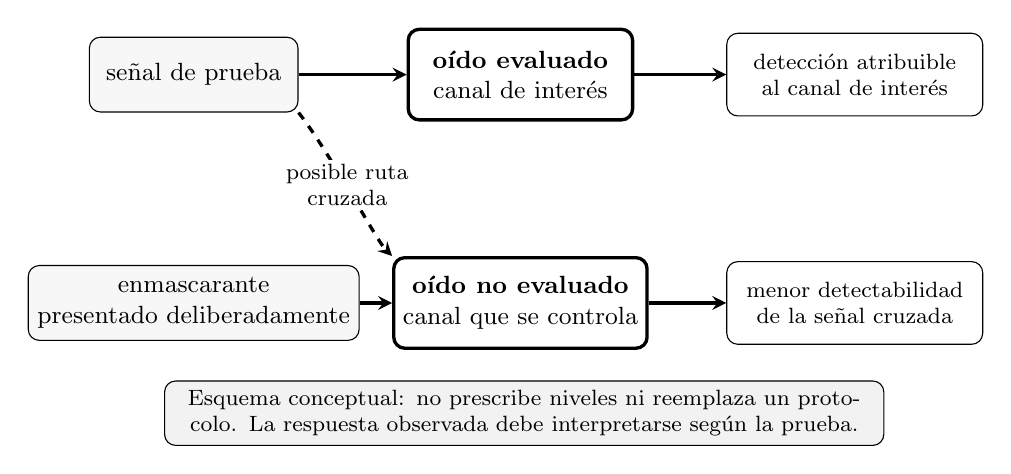
\begin{tikzpicture}[
    x=0.965cm,
    y=1cm,
    >=stealth,
    font=\small,
    senal/.style={
        draw,
        rounded corners,
        minimum width=2.65cm,
        minimum height=0.95cm,
        align=center,
        fill=black!3
    },
    oido/.style={
        draw,
        very thick,
        rounded corners,
        minimum width=2.85cm,
        minimum height=1.15cm,
        align=center
    },
    resultado/.style={
        draw,
        rounded corners,
        minimum width=3.25cm,
        minimum height=1.05cm,
        align=center,
        font=\footnotesize
    }
]
    \node[senal] (prueba) at (1.70,4.25)
        {señal de prueba};
    \node[senal] (masker) at (1.70,1.35)
        {enmascarante\\presentado deliberadamente};

    \node[oido] (evaluado) at (6.00,4.25)
        {\textbf{oído evaluado}\\
         canal de interés};
    \node[oido] (no-evaluado) at (6.00,1.35)
        {\textbf{oído no evaluado}\\
         canal que se controla};

    \node[resultado] (deteccion) at (10.40,4.25)
        {detección atribuible\\
         al canal de interés};
    \node[resultado] (cruzada) at (10.40,1.35)
        {menor detectabilidad\\
         de la señal cruzada};

    \draw[->,very thick] (prueba) -- (evaluado);
    \draw[->,very thick] (evaluado) -- (deteccion);

    \draw[->,very thick,dashed]
        (prueba.south east)
        .. controls (3.50,3.25) and (4.10,2.15) ..
        (no-evaluado.north west);
    \node[
        fill=white,
        inner sep=1.5pt,
        align=center,
        font=\footnotesize
    ] at (3.72,2.85)
        {posible ruta\\cruzada};

    \draw[->,very thick] (masker) -- (no-evaluado);
    \draw[->,very thick] (no-evaluado) -- (cruzada);

    \node[
        draw,
        rounded corners,
        fill=black!5,
        align=center,
        font=\footnotesize,
        text width=8.9cm
    ] at (6.05,-0.05)
        {Esquema conceptual: no prescribe niveles ni reemplaza un protocolo.
         La respuesta observada debe interpretarse según la prueba.};
\end{tikzpicture}

    \caption{Esquema funcional del enmascaramiento audiométrico introductorio.
    La señal de prueba se dirige al oído evaluado, pero puede existir una ruta
    cruzada hacia el oído no evaluado. El enmascarante se presenta de manera
    deliberada en este último para disminuir allí la detectabilidad de la
    señal cruzada. La figura no establece indicaciones, niveles, incrementos
    ni criterios de finalización. Elaboración propia.}
    \label{fig:u10-enmascaramiento-audiometrico}
\end{figure}

La acufenometría puede incluir la comparación de tonos o ruidos con la
percepción referida por la persona y la determinación de medidas de
enmascaramiento. Su interpretación y el uso terapéutico de sonidos requieren
evaluación profesional, protocolo y evidencia clínica específica. Esta unidad
no prescribe un tipo de ruido ni un nivel para tinnitus~\cite{ashaTinnitus}.

\section{Exposición, salud y comunicación}
\label{sec:u10-efectos}

El ruido puede estudiarse en tres planos que conviene mantener separados:
\begin{description}
    \item[\textbf{Exposición física:}] nivel, espectro, duración, repetición y
    condiciones de propagación.
    \item[\textbf{Resultado funcional o perceptual:}] detectabilidad,
    inteligibilidad, molestia, esfuerzo o interferencia con una tarea.
    \item[\textbf{Resultado de salud:}] alteración, síntoma o riesgo evaluado
    en una población y bajo condiciones definidas.
\end{description}

La exposición a determinados niveles y duraciones puede asociarse con
efectos auditivos, como cambios temporales o permanentes de umbral y tinnitus,
y con efectos no auditivos. La magnitud del riesgo depende de la exposición y
de factores individuales y contextuales; una medición aislada no establece
por sí sola un diagnóstico ni una relación causal individual~\cite{whoEnvNoise2018,nioshNoise1998}.

El ruido puede interferir con la comunicación oral y con tareas que
requieren atención. El resultado depende, entre otros factores, de la SNR, el
contenido espectral y temporal, la reverberación, la distancia, las
características del habla, la tarea y el oyente~\cite{whoEnvNoise2018,nioshNoise1998}.

Las alteraciones, los estudios y la rehabilitación se desarrollaron en la
\nameref{chap:unidad-8}. Esta unidad aporta descriptores de la exposición,
pero no reemplaza una evaluación clínica ni ofrece consejo médico individual.

\subsection{Cómo leer recomendaciones y normas}
\label{sec:u10-normativa}

No todo documento que contiene decibeles cumple la misma función:
\begin{center}
\begin{tabular}{|
    >{\raggedright\arraybackslash}p{0.24\textwidth}|
    >{\raggedright\arraybackslash}p{0.31\textwidth}|
    >{\raggedright\arraybackslash}p{0.33\textwidth}|}
    \hline
    \textbf{Tipo de documento} & \textbf{Pregunta principal} &
    \textbf{Dato imprescindible} \\
    \hline
    Norma de medición & ¿Cómo medir, calcular e informar una magnitud? &
    Edición, instrumento, ponderaciones, intervalo y procedimiento. \\
    \hline
    Guía de salud & ¿Qué asociación o recomendación se propone para una
    población y un resultado? &
    Organismo, población, indicador, evidencia y alcance. \\
    \hline
    Criterio legal u ocupacional & ¿Qué obligación o acción corresponde en
    una jurisdicción? &
    Autoridad, jurisdicción, vigencia, jornada, regla de intercambio y
    excepciones. \\
    \hline
\end{tabular}
\end{center}

Por lo tanto, no se debe atribuir a una norma de medición un límite sanitario
que no establece, ni combinar el nivel admisible de un documento con la regla
de intercambio de otro.

Antes de aplicar recomendaciones de exposición o seleccionar
protección auditiva deben consultarse las normas técnicas, la legislación y
las guías vigentes para la jurisdicción y la población correspondientes. En
Argentina, cualquier referencia ocupacional debe comprobarse en las fuentes
oficiales actuales y no trasladarse automáticamente a ambientes comunitarios,
educativos o clínicos~\cite{argentinaLey19587,argentinaDecreto351,argentinaResolucion85}.

Los límites de ruido admisible para salas de prueba audiométrica
dependen de la prueba, la vía, el transductor, las frecuencias evaluadas y el
documento técnico aplicable. Un único valor global en \(\mathrm{dB(A)}\) no
garantiza por sí solo que una cabina sea adecuada~\cite{iso8253_1_2010,ansiS31_2023}. Véase también la
sección~\ref{sec:u9-ruido-cabina}.

\section{Control en la fuente, el trayecto y el receptor}
\label{sec:u10-control}

Controlar ruido significa modificar una cadena física para reducir la
exposición o la interferencia relevante. Conviene comenzar por identificar la
fuente, seguir el trayecto de transmisión y definir el receptor o la tarea que
se desea proteger.

\begin{description}
    \item[\textbf{Fuente:}] reducir la generación mediante selección,
    mantenimiento, ajuste de operación, encapsulado o sustitución del proceso,
    según el caso.
    \item[\textbf{Trayecto:}] aumentar distancia, interponer cerramientos o
    barreras, controlar aberturas, desacoplar vibraciones o acondicionar el
    recinto cuando corresponda.
    \item[\textbf{Receptor:}] limitar el tiempo de exposición, organizar la
    tarea, alejar al receptor o emplear protección auditiva seleccionada y
    verificada para la situación.
\end{description}

Las jerarquías de control ocupacional suelen priorizar la eliminación
o reducción en la fuente y las medidas de ingeniería antes que las medidas
administrativas y la protección personal. La formulación exacta debe
verificarse en el marco normativo vigente~\cite{nioshHierarchy2024}.

La figura~\ref{fig:u10-control-ftr} organiza las medidas según el eslabón sobre
el que actúan. La reducción es el resultado comparado; absorción, aislamiento,
cancelación activa y protección describen mecanismos o intervenciones.

% Texto alternativo: una cadena horizontal conecta fuente, trayecto y receptor.
% Bajo la fuente aparecen acciones sobre la generación; bajo el trayecto se
% separan transmisión y reflexiones; bajo el receptor aparecen distancia,
% tiempo, organización y protección. Las tres familias de acciones apuntan a
% un bloque común que presenta la reducción como resultado comparado entre
% condiciones.
\begin{figure}[htbp]
    \centering
    % Propósito: organizar las medidas de control según el eslabón físico sobre el
% que actúan y separar transmisión, reflexión y protección.
% Origen: sección \ref{sec:u10-control}; esquema cualitativo sin prestaciones.
% Descripción accesible: una cadena conecta fuente, trayecto y receptor. Debajo
% de la fuente aparecen reducción de generación y encapsulado; debajo del
% trayecto se separan transmisión y reflexiones; debajo del receptor aparecen
% distancia, tiempo, organización y protección. Las tres familias de acciones
% apuntan a un bloque común: el resultado se evalúa como cambio de una métrica
% entre condiciones declaradas.
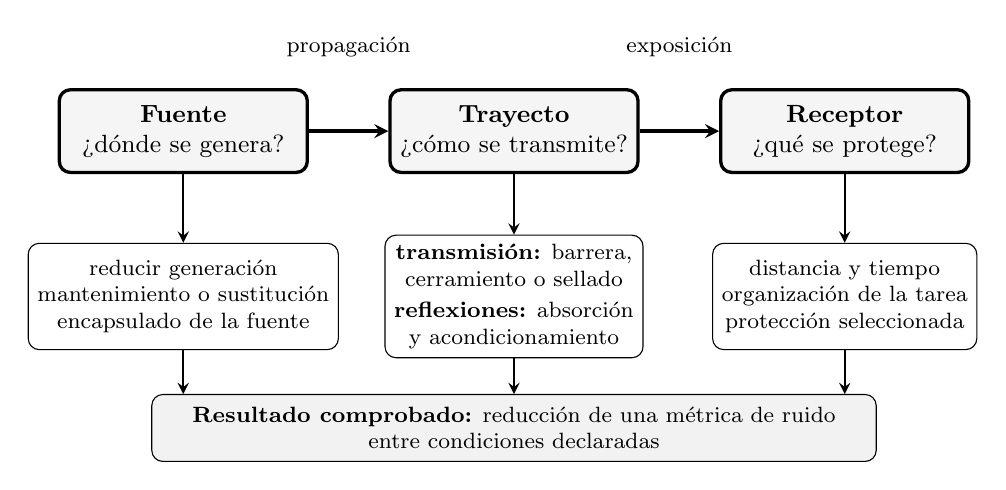
\begin{tikzpicture}[
    x=1cm,
    y=1cm,
    >=stealth,
    font=\small,
    etapa/.style={
        draw,
        rounded corners,
        very thick,
        minimum width=3.15cm,
        minimum height=1.05cm,
        align=center,
        fill=black!4
    },
    accion/.style={
        draw,
        rounded corners,
        minimum width=3.15cm,
        minimum height=1.35cm,
        align=center,
        font=\footnotesize
    },
    resultado/.style={
        draw,
        rounded corners,
        minimum width=9.20cm,
        minimum height=0.85cm,
        align=center,
        fill=black!5,
        font=\footnotesize
    }
]
    \node[etapa] (fuente) at (1.90,4.25)
        {\textbf{Fuente}\\¿dónde se genera?};
    \node[etapa] (trayecto) at (6.10,4.25)
        {\textbf{Trayecto}\\¿cómo se transmite?};
    \node[etapa] (receptor) at (10.30,4.25)
        {\textbf{Receptor}\\¿qué se protege?};

    \draw[->,very thick] (fuente) -- (trayecto)
        node[midway,above=23pt,font=\footnotesize] {propagación};
    \draw[->,very thick] (trayecto) -- (receptor)
        node[midway,above=23pt,font=\footnotesize] {exposición};

    \node[accion] (accion-f) at (1.90,2.15)
        {reducir generación\\
         mantenimiento o sustitución\\
         encapsulado de la fuente};
    \node[accion] (accion-t) at (6.10,2.15)
        {\textbf{transmisión:} barrera,\\
         cerramiento o sellado\\[2pt]
         \textbf{reflexiones:} absorción\\
         y acondicionamiento};
    \node[accion] (accion-r) at (10.30,2.15)
        {distancia y tiempo\\
         organización de la tarea\\
         protección seleccionada};

    \draw[->,thick] (fuente) -- (accion-f);
    \draw[->,thick] (trayecto) -- (accion-t);
    \draw[->,thick] (receptor) -- (accion-r);

    \node[resultado] (resultado) at (6.10,0.48)
        {\textbf{Resultado comprobado:} reducción de una métrica de ruido\\
         entre condiciones declaradas};
    \draw[->,thick] (accion-f.south) -- (1.90,0.91);
    \draw[->,thick] (accion-t.south) -- (6.10,0.91);
    \draw[->,thick] (accion-r.south) -- (10.30,0.91);
\end{tikzpicture}

    \caption{Mapa de control en la cadena fuente--trayecto--receptor. Las
    acciones sobre la fuente modifican la generación; las del trayecto actúan
    sobre transmisión o reflexiones; y las del receptor modifican la
    exposición o la tarea. ``Reducción de ruido'' designa el cambio de una
    métrica entre condiciones declaradas, no un mecanismo único. Esquema
    cualitativo de elaboración propia.}
    \label{fig:u10-control-ftr}
\end{figure}

\subsection{Términos que no deben confundirse}

\begin{description}
    \item[\textbf{Reducción de ruido:}] resultado general: disminución de una
    métrica de ruido entre dos condiciones declaradas.
    \item[\textbf{Absorción:}] disminución de la energía reflejada por una
    superficie; puede modificar la reverberación, pero no equivale a aislar.
    \item[\textbf{Aislamiento:}] reducción de la transmisión entre recintos o
    a través de un elemento constructivo.
    \item[\textbf{Cancelación activa:}] superposición controlada de una señal
    secundaria para reducir la presión en una región y bajo condiciones
    específicas; no elimina universalmente el campo sonoro.
    \item[\textbf{Protección auditiva:}] dispositivo y programa
    destinados a reducir la exposición que llega al oído. Su desempeño real
    no se obtiene sumando sin más valores declarados por fabricantes; la
    selección y la estimación de la protección requieren el procedimiento
    vigente~\cite{iso4869_2_2018}.
\end{description}

Los principios de absorción, transmisión, aislamiento y cabinas se
desarrollaron en la \nameref{chap:unidad-9}. La cancelación activa se apoya
en la superposición estudiada en la \nameref{chap:unidad-3}.

\paragraph{Ejemplo de reducción.}
Sean \(I_i\) la intensidad inicial e \(I_f\) la intensidad final, ambas
expresadas en vatios por metro cuadrado (\(\mathrm{W/m^2}\)). Sean \(L_i\) y
\(L_f\) sus niveles de intensidad asociados, expresados en decibeles y
calculados respecto de una misma intensidad de referencia. Si
\(I_f=0{,}1I_i\), el cambio de nivel es
\[
L_f-L_i
=10\log_{10}\left(\frac{I_f}{I_i}\right)
=10\log_{10}(0{,}1)=-10\,\mathrm{dB}.
\]
Si definimos la reducción positiva como
\(R=L_i-L_f\), entonces
\(R=10\,\mathrm{dB}\). Debe declararse dónde se midió cada intensidad y qué
otras condiciones se mantuvieron constantes.

\section{Relación con la Fonoaudiología}
\label{sec:u10-fonoaudiologia}

La caracterización del ruido permite formular preguntas relevantes sin saltar
directamente a conclusiones clínicas:
\begin{itemize}
    \item en una evaluación auditiva, ayuda a describir el ambiente y las
    señales de prueba;
    \item en voz y habla, permite analizar la SNR y la interferencia con la
    comunicación;
    \item en salud ocupacional y comunitaria, permite describir la exposición
    con la métrica elegida; y
    \item en el diseño de espacios, orienta la elección entre actuar sobre la
    fuente, el trayecto o el receptor.
\end{itemize}

La contribución fonoaudiológica no consiste en reemplazar la medición técnica,
la normativa o el diagnóstico por una impresión general. Consiste en conectar
las propiedades físicas de la señal con la tarea comunicativa o auditiva,
reconociendo los límites de cada inferencia.

\section{Errores frecuentes}
\label{sec:u10-errores}

\begin{itemize}
    \item \textbf{``Ruido'' significa siempre sonido intenso.} No. Puede
    tratarse de una señal de bajo nivel que interfiere con una tarea.
    \item \textbf{Aleatorio significa no medible.} No. No se predice cada
    muestra, pero se describen propiedades estadísticas y espectrales.
    \item \textbf{Estacionario significa constante muestra a muestra.} No.
    Pueden variar los valores instantáneos mientras ciertas estadísticas
    permanecen estables.
    \item \textbf{Media y RMS son equivalentes.} No. La media conserva el
    signo; el RMS se obtiene a partir de cuadrados.
    \item \textbf{Ruido blanco significa igual energía por octava.} No. Posee
    densidad constante por hertz; el rosa ideal posee contenido constante por
    octava.
    \item \textbf{\(L_{\mathrm{max}}\) y \(L_{\mathrm{peak}}\) son
    intercambiables.} No. Dependen de detectores distintos.
    \item \textbf{\(L_{\mathrm{eq}}\) es el promedio aritmético de los
    decibeles.} No. Se promedian primero cantidades lineales proporcionales al
    valor cuadrático.
    \item \textbf{\(L_{90}\) siempre es el ruido de fondo.} No. Es un
    percentil; su uso como descriptor de fondo depende del contexto.
    \item \textbf{Enmascarar equivale a proteger el oído.} No. Son objetivos y
    procedimientos diferentes.
    \item \textbf{Absorber equivale a aislar.} No. La absorción modifica
    reflexiones; el aislamiento limita transmisión entre espacios.
    \item \textbf{Un número en \(\mathrm{dB(A)}\) basta para decidir
    cumplimiento o riesgo.} No. Faltan duración, procedimiento, norma,
    población y jurisdicción.
\end{itemize}

\section{Síntesis}
\label{sec:u10-sintesis}

\begin{itemize}
    \item El sonido es un fenómeno físico; ruido es una categoría que puede
    referirse a una valoración contextual, una componente no deseada o una
    señal de ensayo.
    \item Las señales determinísticas se predicen a partir de un modelo; las
    aleatorias se describen mediante realizaciones y estadísticas.
    \item Estacionariedad y clasificación temporal dependen del intervalo de
    observación. Continuo, fluctuante, intermitente e impulsivo describen
    aspectos distintos.
    \item El valor medio, el RMS, la varianza y la distribución responden
    preguntas diferentes.
    \item La densidad espectral \(S_{pp}(f)\), en
    \(\mathrm{Pa^2/Hz}\), se integra sobre una banda para obtener presión
    cuadrática media.
    \item El ruido blanco posee densidad constante por hertz; el rosa ideal,
    contenido constante por octava.
    \item Los ruidos con forma espectral vocal y de banda estrecha deben
    definirse mediante espectro, límites, ancho de banda y nivel, no solo por
    su nombre.
    \item Nivel instantáneo, máximo, de pico y equivalente no son
    intercambiables.
    \item El ruido de fondo aparece como interferencia; un enmascarante se
    presenta deliberadamente. Ninguno equivale por sí mismo a protección
    auditiva.
    \item Las recomendaciones de exposición y protección requieren fuentes
    vigentes y no constituyen consejo médico individual.
    \item El control se organiza en fuente, trayecto y receptor, diferenciando
    reducción, absorción, aislamiento, cancelación activa y protección.
\end{itemize}

\section{Ejercicios y autoevaluación}
\label{sec:u10-ejercicios}

\subsection*{Preguntas conceptuales}

\begin{enumerate}[label=\textbf{C\arabic*.},leftmargin=*]
    \item Explique por qué una misma señal puede ser sonido para quien desea
    escucharla y ruido respecto de otra tarea, sin que cambien sus propiedades
    físicas.
    \item Compare una sinusoide ideal cuyos parámetros son conocidos con un
    registro aleatorio de tránsito. Indique qué puede predecirse en cada
    instante y qué debe describirse mediante propiedades estadísticas.
    \item ¿Puede una señal estacionaria cambiar muestra a muestra? Explique
    por qué la respuesta depende también del intervalo de observación.
    \item Distinga ruido continuo, fluctuante, intermitente e impulsivo.
    Explique por qué estas categorías no son necesariamente excluyentes.
    \item Diferencie valor medio, valor eficaz o RMS y varianza. Indique sus
    unidades para una señal de presión acústica expresada en pascales
    \((\mathrm{Pa})\).
    \item ¿Qué información aporta la distribución de amplitudes que no aporta
    por sí solo el RMS?
    \item Explique la diferencia entre densidad espectral, expresada en
    \(\mathrm{Pa^2/Hz}\), y valor cuadrático medio contenido en una banda,
    expresado en \(\mathrm{Pa^2}\).
    \item Compare ruido blanco y ruido rosa ideales: ¿qué magnitud se mantiene
    constante por hertz y cuál por octava?
    \item Distinga nivel instantáneo, nivel máximo, nivel de pico y nivel
    equivalente. Indique al menos un dato que debe acompañar a cada lectura.
    \item Diferencie ruido de fondo y señal enmascarante. Luego explique por
    qué el enmascaramiento clínico no equivale a protección auditiva.
\end{enumerate}

\subsection*{Identificación e interpretación de gráficos}

\begin{enumerate}[label=\textbf{V\arabic*.},leftmargin=*]
    \item Observe la Figura~\ref{fig:u10-realizaciones-temporales}.
    \begin{enumerate}
        \item Asigne a cada panel una o más categorías temporales.
        \item Indique qué codifican los ejes y sus unidades.
        \item Explique por qué los trazos no permiten inferir por sí solos un
        efecto perceptual, clínico o sanitario.
    \end{enumerate}

    \item En la Figura~\ref{fig:u10-estadistica-mismo-rms}:
    \begin{enumerate}
        \item identifique los tres descriptores que comparten ambas señales;
        \item señale la diferencia que revelan los histogramas; y
        \item explique por qué observar únicamente el RMS perdería esa
        diferencia.
    \end{enumerate}

    \item Use la Figura~\ref{fig:u10-blanco-rosa-bandas} para relacionar cada
    curva de densidad con sus barras por octava. Explique qué ocurriría, para
    el modelo blanco, al integrar dos bandas con igual ancho en hertz, y qué
    ocurriría, para el modelo rosa, al integrar dos octavas sucesivas.

    \item En la Figura~\ref{fig:u10-conformacion-espectral}:
    \begin{enumerate}
        \item identifique qué transformación produce cada salida;
        \item localice \(f_L\), \(f_c\) y \(f_H\) en el esquema del NBN; y
        \item enumere la información que falta para convertir cada esquema
        cualitativo en una señal de prueba especificada.
    \end{enumerate}

    \item Compare los tres paneles de la
    Figura~\ref{fig:u10-snr-sintetica}.
    \begin{enumerate}
        \item Ordénelos de mayor a menor SNR.
        \item Indique qué componente se mantiene fija y cuál cambia de escala.
        \item Explique por qué el gráfico no permite predecir directamente la
        inteligibilidad ni la molestia.
    \end{enumerate}

    \item En la Figura~\ref{fig:u10-enmascaramiento-audiometrico}, identifique
    la señal de prueba, el enmascarante, el oído evaluado, el oído no evaluado
    y la posible ruta cruzada. Explique por qué el esquema no constituye un
    protocolo de enmascaramiento.

    \item Use la Figura~\ref{fig:u10-control-ftr} para ubicar estas acciones:
    mantenimiento de un equipo, sellado de una abertura, absorción de
    reflexiones interiores y limitación del tiempo de exposición. Explique por
    qué la reducción de ruido aparece como resultado de comparar condiciones
    y no como un cuarto mecanismo independiente.
\end{enumerate}

\subsection*{Ejercicios numéricos guiados}

\begin{enumerate}[label=\textbf{G\arabic*.},leftmargin=*]
    \item Para las cuatro muestras de presión
    \(-3,-1,1,3\,\mathrm{mPa}\):
    \begin{enumerate}
        \item calcule el valor medio \(\overline p\), expresado en
        milipascales \((\mathrm{mPa})\);
        \item calcule el promedio de los cuadrados y
        \(p_{\mathrm{rms}}\), expresado en \(\mathrm{mPa}\);
        \item calcule \(\sigma_p^2\), expresada en
        \(\mathrm{mPa^2}\), y compruebe la
        ecuación~\eqref{eq:u10-identidad-estadistica}.
    \end{enumerate}

    \item Para las cuatro muestras
    \(1,1,1,1\,\mathrm{mPa}\), repita el cálculo de
    \(\overline p\), \(p_{\mathrm{rms}}\) y \(\sigma_p^2\). Explique por qué
    un RMS distinto de \(0\,\mathrm{mPa}\) es compatible con varianza nula.

    \item Una densidad espectral constante vale
    \(2{,}5\times10^{-9}\,\mathrm{Pa^2/Hz}\) entre
    \(f_L=200\,\mathrm{Hz}\) y \(f_H=600\,\mathrm{Hz}\).
    \begin{enumerate}
        \item calcule el ancho de banda en hertz \((\mathrm{Hz})\);
        \item obtenga \(p_{B,\mathrm{rms}}^2\), expresado en
        \(\mathrm{Pa^2}\); y
        \item calcule \(p_{B,\mathrm{rms}}\), expresado en pascales
        \((\mathrm{Pa})\).
    \end{enumerate}

    \item Un ruido de banda estrecha posee
    \(f_L=900\,\mathrm{Hz}\) y \(f_H=1100\,\mathrm{Hz}\).
    \begin{enumerate}
        \item calcule el ancho \(B\), expresado en hertz \((\mathrm{Hz})\);
        \item indique qué información adicional pediría antes de utilizarlo
        como señal de prueba.
    \end{enumerate}

    \item Se consideran dos intervalos de igual duración, cuyos niveles son
    \[
        L_{A\mathrm{eq},1}=70\,\mathrm{dB(A)}
        \qquad\text{y}\qquad
        L_{A\mathrm{eq},2}=80\,\mathrm{dB(A)}.
    \]
    \begin{enumerate}
        \item convierta cada nivel en la cantidad relativa
        \(10^{L_{A\mathrm{eq}}/10}\);
        \item promedie esas cantidades; y
        \item calcule el nivel equivalente del intervalo conjunto. Exprese el
        resultado en \(\mathrm{dB(A)}\).
    \end{enumerate}
\end{enumerate}

\subsection*{Ejercicios numéricos autónomos}

\begin{enumerate}[label=\textbf{A\arabic*.},leftmargin=*]
    \item Para las muestras de presión
    \(0,2,2,4\,\mathrm{mPa}\), calcule
    \(\overline p\), \(p_{\mathrm{rms}}\) y \(\sigma_p^2\), con sus unidades,
    y verifique la ecuación~\eqref{eq:u10-identidad-estadistica}.

    \item Una señal sintética posee
    \(S_{pp}(f)=9{,}0\times10^{-10}\,\mathrm{Pa^2/Hz}\) entre
    \(500\,\mathrm{Hz}\) y \(2500\,\mathrm{Hz}\), y densidad nula fuera de esa
    banda. Calcule \(p_{\mathrm{rms}}^2\), expresado en
    \(\mathrm{Pa^2}\); \(p_{\mathrm{rms}}\), expresado en
    \(\mathrm{Pa}\); y \(L_p\), expresado en \(\mathrm{dB\,SPL}\), con
    \(p_0=20\,\mathrm{\mu Pa}\).

    \item Una señal de interés posee
    \(L_{\text{señal}}=68\,\mathrm{dB\,SPL}\) y el ruido de fondo
    \(L_{\text{ruido}}=73\,\mathrm{dB\,SPL}\), medidos en la misma posición,
    banda e intervalo. Calcule la SNR, expresada en decibeles
    \((\mathrm{dB})\), e interprete el signo sin convertirlo en una predicción
    perceptual.

    \item Tres intervalos consecutivos de \(10\,\mathrm{min}\) poseen
    \(L_{A\mathrm{eq}}=74\,\mathrm{dB(A)}\),
    \(78\,\mathrm{dB(A)}\) y \(82\,\mathrm{dB(A)}\). Calcule
    \(L_{A\mathrm{eq},30\,\mathrm{min}}\), expresado en \(\mathrm{dB(A)}\), y compárelo
    con el promedio aritmético de los tres niveles.
\end{enumerate}

\subsection*{Aplicaciones a Fonoaudiología}

\begin{enumerate}[label=\textbf{F\arabic*.},leftmargin=*]
    \item En un aula se desea analizar la inteligibilidad de una conversación.
    Hay ventilación continua y portazos ocasionales. Identifique la señal de
    interés, el ruido de fondo y los eventos impulsivos. Indique qué
    descriptores físicos registraría sin afirmar a partir de ellos un
    resultado perceptual.

    \item Una aplicación telefónica sin calibración informa un nivel dentro de
    un consultorio. Explique para qué podría servir como observación
    exploratoria y por qué no basta para certificar cumplimiento normativo.

    \item Para una cabina audiométrica, explique por qué un único valor global
    en \(\mathrm{dB(A)}\) no permite decidir si todas las pruebas son válidas.
    Enumere la información técnica que debería acompañar la evaluación.

    \item Un consultorio recibe ruido por una abertura y además posee mucha
    reverberación. Proponga una intervención sobre la transmisión y otra sobre
    las reflexiones internas. Nombre correctamente cada mecanismo y señale qué
    resultado debería medirse antes y después.

    \item Compare enmascaramiento audiométrico, cancelación activa y
    protección auditiva según su objetivo, la función de la señal introducida
    y el receptor o región sobre la que actúan.
\end{enumerate}

\subsection*{Pregunta integradora}

\begin{enumerate}[label=\textbf{I\arabic*.},leftmargin=*]
    \item Un consultorio próximo a una avenida contiene un equipo de
    climatización continuo y recibe portazos intermitentes del pasillo. Allí
    se realizan tareas de comunicación y evaluaciones auditivas. Organice un
    plan de caracterización que incluya evolución temporal, estadística,
    espectro, nivel equivalente, máximos o picos y SNR. Distinga ruido de
    fondo de señal enmascarante; proponga controles en fuente, trayecto y
    receptor; e indique qué decisiones requieren medición calibrada, norma o
    protocolo clínico vigente.
\end{enumerate}

\subsection*{Errores frecuentes y distractores razonables}

Para cada afirmación, indique si es correcta, incorrecta o incompleta y
justifique.

\begin{enumerate}[label=\textbf{D\arabic*.},leftmargin=*]
    \item ``El ruido rosa tiene menos contenido en cada octava a medida que
    aumenta la frecuencia''.
    \item ``Si dos señales tienen el mismo \(L_{A\mathrm{eq},T}\), producen los mismos
    picos y el mismo efecto''.
    \item ``La respuesta temporal \emph{Impulse} mide directamente
    \(L_{\mathrm{peak}}\)''.
    \item ``Un NBN siempre ocupa un tercio de octava''.
    \item ``Si \(L_{90,T}\) es bajo, la sala cumple cualquier requisito
    audiométrico''.
\end{enumerate}

\section{Soluciones y orientaciones}
\label{sec:u10-respuestas}

\subsection*{Preguntas conceptuales}

\begin{enumerate}[label=\textbf{C\arabic*.},leftmargin=*]
    \item ``Ruido'' incorpora la relación con una tarea o una valoración,
    mientras que presión, nivel, espectro y duración describen propiedades
    físicas de la señal. Cambiar la tarea no modifica por sí solo esas
    propiedades.
    \item En la sinusoide ideal, amplitud, frecuencia, fase y duración permiten
    predecir el valor en cada instante. En el registro aleatorio no se predice
    cada muestra; se caracterizan, por ejemplo, su media, RMS, distribución y
    densidad espectral.
    \item Sí. La estacionariedad se refiere a la estabilidad de las
    propiedades estadísticas elegidas, no a un valor instantáneo constante.
    Además, una señal puede parecer estable en una ventana breve y cambiar al
    ampliar el intervalo de observación.
    \item El ruido continuo permanece durante el intervalo; el fluctuante
    permanece, pero cambia apreciablemente de nivel; el intermitente alterna
    actividad y pausas relativas; y el impulsivo contiene eventos breves y
    abruptos. Una serie de golpes separados, por ejemplo, puede ser impulsiva
    e intermitente.
    \item La media conserva el signo y el RMS cuantifica el tamaño cuadrático;
    ambos se expresan en \(\mathrm{Pa}\). La varianza cuantifica la dispersión
    respecto de la media y se expresa en \(\mathrm{Pa^2}\).
    \item La distribución muestra con qué frecuencia aparecen los valores,
    incluida la presencia de valores extremos. Dos señales con el mismo RMS
    pueden tener distribuciones distintas.
    \item La densidad expresa valor cuadrático medio por unidad de ancho de
    banda, en \(\mathrm{Pa^2/Hz}\). Su integral sobre una banda produce el
    valor cuadrático medio contenido en ella, en \(\mathrm{Pa^2}\).
    \item El blanco ideal mantiene constante \(S_{pp}(f)\) por hertz. El rosa
    ideal mantiene constante el valor cuadrático medio integrado en cada
    octava.
    \item \(L(t)\) es una indicación instantánea y requiere las ponderaciones
    frecuencial y temporal. \(L_{\mathrm{max}}\) es la mayor indicación y
    requiere además un intervalo de búsqueda. \(L_{\mathrm{peak}}\) se asocia
    con el extremo instantáneo de presión y requiere detector, rango y
    procedimiento. \(L_{\mathrm{eq},T}\) conserva el promedio cuadrático y
    requiere la duración \(T\) y la ponderación frecuencial.
    \item El ruido de fondo es una interferencia presente en el entorno o la
    medición; el enmascarante se introduce deliberadamente. En una prueba, el
    enmascaramiento modifica la detectabilidad; la protección auditiva busca
    reducir la exposición que llega al oído.
\end{enumerate}

\subsection*{Identificación e interpretación de gráficos}

\begin{enumerate}[label=\textbf{V\arabic*.},leftmargin=*]
    \item Los paneles representan, respectivamente, ruido continuo
    aproximadamente estable, continuo fluctuante, intermitente e impulsivo.
    Los ejes muestran tiempo en segundos \((\mathrm{s})\) y presión acústica
    en pascales \((\mathrm{Pa})\). Las formas son realizaciones sintéticas:
    sin métrica de exposición, contexto, tarea y receptor no permiten
    inferir un efecto perceptual, clínico o sanitario.

    \item Ambas señales comparten
    \(\overline p=0\,\mathrm{mPa}\),
    \(p_{\mathrm{rms}}=1\,\mathrm{mPa}\) y
    \(\sigma_p^2=1\,\mathrm{mPa^2}\). El histograma de A contiene valores
    continuos, mientras B solo adopta \(-1\,\mathrm{mPa}\) y
    \(+1\,\mathrm{mPa}\). El RMS reduce cada registro a un único valor y no
    conserva esa distribución.

    \item La densidad horizontal corresponde al blanco; al integrar bandas con
    igual ancho en hertz se obtiene igual valor cuadrático medio. La curva
    proporcional a \(1/f\) corresponde al rosa; su integral tiene el mismo
    valor en octavas sucesivas. Las barras muestran que, por octava, el
    contenido blanco aumenta con el ancho en hertz y el rosa permanece
    constante.

    \item En la cadena superior, un filtro con respuesta objetivo especificada
    produce ruido con forma espectral vocal. En la inferior, un filtro
    pasabanda produce NBN; \(f_L\) y \(f_H\) delimitan la banda y \(f_c\)
    identifica su centro. Para especificar las señales faltan, según el caso,
    espectro objetivo, límites y ancho de banda, pendientes, nivel, equipo,
    transductor, calibración y procedimiento.

    \item El orden de mayor a menor es
    \(+12\,\mathrm{dB}\), \(0\,\mathrm{dB}\) y
    \(-6\,\mathrm{dB}\). Se mantienen la señal de interés y la realización de
    ruido; cambia la escala RMS del ruido. La SNR describe una relación física,
    pero la inteligibilidad y la molestia dependen además del espectro, el
    tiempo, el entorno, la tarea y el oyente.

    \item La señal de prueba se dirige al oído evaluado y la ruta discontinua
    representa una posible llegada al oído no evaluado. El enmascarante se
    presenta deliberadamente en este último. Como la figura no fija
    indicaciones, niveles, incrementos, transductores ni criterios de
    finalización, no constituye un protocolo.

    \item El mantenimiento actúa sobre la fuente; el sellado, sobre la
    transmisión en el trayecto; la absorción, sobre las reflexiones del
    trayecto; y el límite temporal, sobre la exposición del receptor. La
    reducción es el cambio de una métrica entre las condiciones anterior y
    posterior a una o más acciones.
\end{enumerate}

\subsection*{Ejercicios numéricos guiados}

\begin{enumerate}[label=\textbf{G\arabic*.},leftmargin=*]
    \item El valor medio es
    \[
        \overline p=\frac{-3-1+1+3}{4}=0\,\mathrm{mPa}.
    \]
    El promedio de los cuadrados es
    \[
        \frac{9+1+1+9}{4}=5\,\mathrm{mPa^2},
    \]
    por lo que
    \[
        p_{\mathrm{rms}}=\sqrt{5}\,\mathrm{mPa}
        \approx2{,}24\,\mathrm{mPa},
        \qquad
        \sigma_p^2=5\,\mathrm{mPa^2}.
    \]
    Se verifica que
    \(p_{\mathrm{rms}}^2=5\,\mathrm{mPa^2}
    =\sigma_p^2+\overline p^{\,2}\).

    \item
    \[
        \overline p=1\,\mathrm{mPa},\qquad
        p_{\mathrm{rms}}=1\,\mathrm{mPa},\qquad
        \sigma_p^2=0\,\mathrm{mPa^2}.
    \]
    Todas las muestras se apartan \(0\,\mathrm{mPa}\) de la media, aunque su
    valor y, por lo tanto, su RMS no sean nulos.

    \item El ancho es
    \[
        f_H-f_L=600-200=400\,\mathrm{Hz}.
    \]
    Como la densidad es constante,
    \[
        p_{B,\mathrm{rms}}^2
        =\left(2{,}5\times10^{-9}\,\mathrm{Pa^2/Hz}\right)
        \left(400\,\mathrm{Hz}\right)
        =1{,}0\times10^{-6}\,\mathrm{Pa^2},
    \]
    y
    \[
        p_{B,\mathrm{rms}}
        =1{,}0\times10^{-3}\,\mathrm{Pa}.
    \]

    \item
    \[
        B=f_H-f_L=1100-900=200\,\mathrm{Hz}.
    \]
    Faltan, entre otros datos, \(f_c\), la forma y las pendientes del filtro,
    el nivel, la calibración, el transductor y el procedimiento.

    \item Las cantidades relativas son
    \(10^{70/10}=10^7\) y \(10^{80/10}=10^8\). Por lo tanto,
    \[
        L_{A\mathrm{eq}}
        =10\log_{10}\left(\frac{10^7+10^8}{2}\right)
        \approx77{,}4\,\mathrm{dB(A)}.
    \]
\end{enumerate}

\subsection*{Ejercicios numéricos autónomos}

\begin{enumerate}[label=\textbf{A\arabic*.},leftmargin=*]
    \item
    \[
        \overline p=\frac{0+2+2+4}{4}
        =2\,\mathrm{mPa},
    \]
    \[
        p_{\mathrm{rms}}
        =\sqrt{\frac{0^2+2^2+2^2+4^2}{4}}
        =\sqrt{6}\,\mathrm{mPa}
        \approx2{,}45\,\mathrm{mPa},
    \]
    \[
        \sigma_p^2
        =\frac{
        \left(0-2\right)^2+\left(2-2\right)^2+
        \left(2-2\right)^2+\left(4-2\right)^2}{4}
        =2\,\mathrm{mPa^2}.
    \]
    En efecto,
    \(p_{\mathrm{rms}}^2=6\,\mathrm{mPa^2}
    =2\,\mathrm{mPa^2}+\left(2\,\mathrm{mPa}\right)^2\).

    \item El ancho de banda es \(2000\,\mathrm{Hz}\). Entonces,
    \[
        p_{\mathrm{rms}}^2
        =\left(9{,}0\times10^{-10}\,\mathrm{Pa^2/Hz}\right)
        \left(2000\,\mathrm{Hz}\right)
        =1{,}8\times10^{-6}\,\mathrm{Pa^2},
    \]
    \[
        p_{\mathrm{rms}}
        =\sqrt{1{,}8\times10^{-6}}\,\mathrm{Pa}
        \approx1{,}34\times10^{-3}\,\mathrm{Pa},
    \]
    y
    \[
        L_p
        =20\log_{10}\left(
        \frac{1{,}34\times10^{-3}\,\mathrm{Pa}}
             {20\times10^{-6}\,\mathrm{Pa}}
        \right)
        \approx36{,}5\,\mathrm{dB\,SPL}.
    \]

    \item
    \[
        \mathrm{SNR}
        =L_{\text{señal}}-L_{\text{ruido}}
        =68-73=-5\,\mathrm{dB}.
    \]
    El signo negativo indica que, en las condiciones comparadas, el nivel del
    ruido supera en \(5\,\mathrm{dB}\) al de la señal. No determina por sí
    solo si una persona detectará o comprenderá la señal.

    \item Como los tres intervalos duran \(10\,\mathrm{min}\),
    \[
        L_{A\mathrm{eq},30\,\mathrm{min}}
        =10\log_{10}\left(
        \frac{10^{74/10}+10^{78/10}+10^{82/10}}{3}
        \right)
        \approx79{,}2\,\mathrm{dB(A)}.
    \]
    El promedio aritmético es
    \((74+78+82)/3=78\,\mathrm{dB(A)}\), que no conserva el promedio
    cuadrático y resulta \(1{,}2\,\mathrm{dB}\) menor.
\end{enumerate}

\subsection*{Aplicaciones a Fonoaudiología}

\begin{enumerate}[label=\textbf{F\arabic*.},leftmargin=*]
    \item La conversación es la señal de interés; la ventilación integra el
    ruido de fondo continuo; y los portazos son eventos impulsivos e
    intermitentes. Pueden registrarse espectro, \(L_{\mathrm{eq},T}\),
    \(L_{\mathrm{max}}\), \(L_{\mathrm{peak}}\) y SNR en condiciones
    declaradas. Esas magnitudes no sustituyen una evaluación de
    inteligibilidad.

    \item La aplicación puede ayudar a comparar de manera preliminar momentos
    o lugares si se mantiene el mismo dispositivo y procedimiento. Sin
    calibración, respuesta frecuencial conocida, posición, intervalo,
    ponderaciones e incertidumbre no existe trazabilidad suficiente para
    certificar un límite.

    \item La ponderación A reúne el espectro en un solo valor. La evaluación
    requiere, entre otros datos, niveles por bandas, prueba, vía, transductor,
    frecuencias evaluadas, menor nivel de prueba, posición, calibración y
    documento técnico aplicable.

    \item Sellar o tratar la abertura actúa sobre la transmisión; incorporar
    absorción apropiada actúa sobre las reflexiones y la reverberación. Debe
    compararse antes y después la misma métrica, en la misma posición, banda,
    intervalo y condición de funcionamiento.

    \item El enmascaramiento audiométrico introduce una señal para modificar
    la detectabilidad en el oído no evaluado durante una prueba. La
    cancelación activa introduce una señal secundaria para reducir presión en
    una región y bajo condiciones específicas. La protección auditiva actúa
    sobre la exposición que llega al oído del usuario.
\end{enumerate}

\subsection*{Pregunta integradora}

\begin{enumerate}[label=\textbf{I\arabic*.},leftmargin=*]
    \item Primero se separarían las fuentes: tránsito, climatización y
    portazos. Registros temporales representativos permitirían evaluar
    estacionariedad y clasificar componentes continuas, fluctuantes,
    intermitentes o impulsivas; media, RMS, varianza e histogramas resumirían
    su estadística; y el análisis por bandas describiría su contenido
    frecuencial. \(L_{\mathrm{eq},T}\) resumiría cada intervalo, mientras
    \(L_{\mathrm{max}}\) y \(L_{\mathrm{peak}}\) atenderían extremos con sus
    detectores declarados. Para la comunicación se medirían señal y ruido en
    condiciones comparables y se calcularía la SNR, sin convertirla
    directamente en inteligibilidad.

    El tránsito, la climatización y los portazos pueden integrar el ruido de
    fondo según la tarea. Una señal enmascarante audiométrica, en cambio, se
    introduce deliberadamente. En la fuente podrían revisarse mantenimiento y
    operación; en el trayecto, aberturas, cerramientos, vibraciones y
    reflexiones; y en el receptor, posición, tiempo y organización de la
    tarea. La exactitud de las mediciones requiere instrumentación calibrada.
    La aptitud de una sala y los criterios de exposición requieren documentos
    vigentes; el enmascaramiento durante una prueba requiere un protocolo
    clínico.
\end{enumerate}

\subsection*{Errores frecuentes y distractores razonables}

\begin{enumerate}[label=\textbf{D\arabic*.},leftmargin=*]
    \item Es incorrecta. El rosa ideal mantiene igual valor cuadrático medio
    por octava; disminuye su densidad por hertz al aumentar \(f\).
    \item Es incorrecta. Igual \(L_{A\mathrm{eq},T}\) no implica iguales máximos,
    picos, espectros o evoluciones temporales, y tampoco permite asegurar un
    mismo efecto perceptual o sanitario.
    \item Es incorrecta. Un detector con ponderación temporal
    \emph{Impulse} y un detector de pico realizan operaciones diferentes.
    \item Es incorrecta. Deben declararse sus límites, frecuencia central,
    ancho y pendientes; no existe una fracción de octava universal para todo
    NBN.
    \item Es incorrecta. Faltan al menos el espectro por bandas, la prueba, la
    vía, el transductor, las frecuencias, el procedimiento y el criterio
    técnico aplicable.
\end{enumerate}

\section{Glosario}
\label{sec:u10-glosario}
\begin{description}
    \item[\textbf{Aleatorio:}] proceso cuyos valores instantáneos se describen
    probabilísticamente.
    \item[\textbf{Densidad espectral \(S_{pp}(f)\):}] distribución del valor
    cuadrático medio de la presión por unidad de ancho de banda, expresada en
    \(\mathrm{Pa^2/Hz}\).
    \item[\textbf{Determinístico:}] predecible a partir de un modelo y sus
    parámetros.
    \item[\textbf{Distribución:}] descripción de la frecuencia o probabilidad
    con que aparecen los valores de una variable.
    \item[\textbf{Enmascarante:}] señal presentada para disminuir la
    detectabilidad de otra.
    \item[\textbf{Estacionario:}] proceso cuyas propiedades estadísticas
    elegidas permanecen estables frente a desplazamientos temporales dentro
    del intervalo considerado.
    \item[\textbf{\(L_{\mathrm{eq},T}\):}] nivel equivalente durante el
    intervalo \(T\).
    \item[\textbf{\(L_{\mathrm{max}}\):}] mayor nivel indicado por un detector
    durante un intervalo.
    \item[\textbf{\(L_{\mathrm{peak}}\):}] nivel asociado con el extremo
    instantáneo de presión registrado por un detector de pico.
    \item[\textbf{NBN:}] ruido de banda estrecha, definido por su banda,
    espectro, nivel y condiciones de generación.
    \item[\textbf{RMS:}] raíz cuadrada del promedio de los cuadrados de una
    señal.
    \item[\textbf{Ruido blanco:}] modelo con densidad espectral constante por
    hertz dentro de una banda declarada.
    \item[\textbf{Ruido de fondo:}] componentes no deseadas presentes durante
    una medición o tarea, definidas según el contexto.
    \item[\textbf{Ruido rosa:}] modelo cuya densidad es inversamente
    proporcional a la frecuencia y que posee igual contenido cuadrático medio
    por octava dentro de una banda declarada.
    \item[\textbf{Varianza:}] promedio del cuadrado de las diferencias
    respecto de la media.
\end{description}

\section{Fuentes externas y alcance documental}
\label{sec:u10-fuentes}

La revisión bibliográfica evaluó los once bloques que estaban marcados con
\verb|\verify{...}|. Se utilizaron, según el caso:
\begin{itemize}
    \item normas técnicas vigentes para terminología, instrumentación,
    audiometría, señales enmascarantes y ruido admisible en salas de prueba;
    \item normativa oficial de la jurisdicción para exposición ocupacional y
    selección de protección;
    \item guías sanitarias vigentes para efectos auditivos y no auditivos; y
    \item bibliografía clínica primaria o guías profesionales para
    enmascaramiento audiométrico, acufenometría y uso terapéutico de sonidos.
\end{itemize}

Las once afirmaciones quedaron respaldadas y se retiraron sus marcas
editoriales. La legislación ocupacional citada corresponde a la jurisdicción
argentina declarada; las guías sanitarias y las normas técnicas conservan sus
propios dominios de aplicación y no se combinan para crear un límite
universal.
